\chapter{Billing Customers}
\label{chap:billingapp}

This example is adapted from the first working Gantry app that did anything
useful.  It was written by Tim Keefer to track his consulting invoices
and appears in a slightly modified form in Bigtop::Docs::Tutorial.  The
version here is very similar to the one in that document, but I've
updated it to our current notions of best practices.

If you are like me, you work for a paycheck.  Perhaps once or twice a year
you do some side work that needs an invoice.  If so, you might do what I
do and type that invoice into a text editor and send it via email.  The
date on the email and a quick check of bank deposits is enough to track it.
But, if you have a few more side jobs, manual invoicing starts to break down.
Hence our case study for this chapter: a billing system for occasional
consultants or landlords with a few tenents who owe them for utilities.

For the purposes of discussion, for the rest of the chapter, I'll pretend
to be a high powered consultant who has too many clients to track by hand.

\section{A Billing Data Model}

As I asserted in Chapter \ref{chap:simpleex}, most web apps are database
front ends.  Our billing app will be no different.  So, let's begin
with the data model.  There are five tables:

\begin{tabular}{l|l}
Table Name          & Purpose                                             \\
\hline
\verb+customers+    & People who occasionally owe me money                \\
\verb+my_companies+ & Names I call myself when doing business             \\
\verb+invoices+     & Bills customers receive in email and eventually pay \\
\verb+line_items+   & Tasks listed on invoices                            \\
\verb+status+       & A code table describing invoice statuses
\end{tabular}

Figure \ref{fig:billing_model} shows all the fields in these tables, but
it was made long ago.  Some of the field names have been changed to
reflect better practices.  This mostly affects the foreign keys.

\begin{figure}
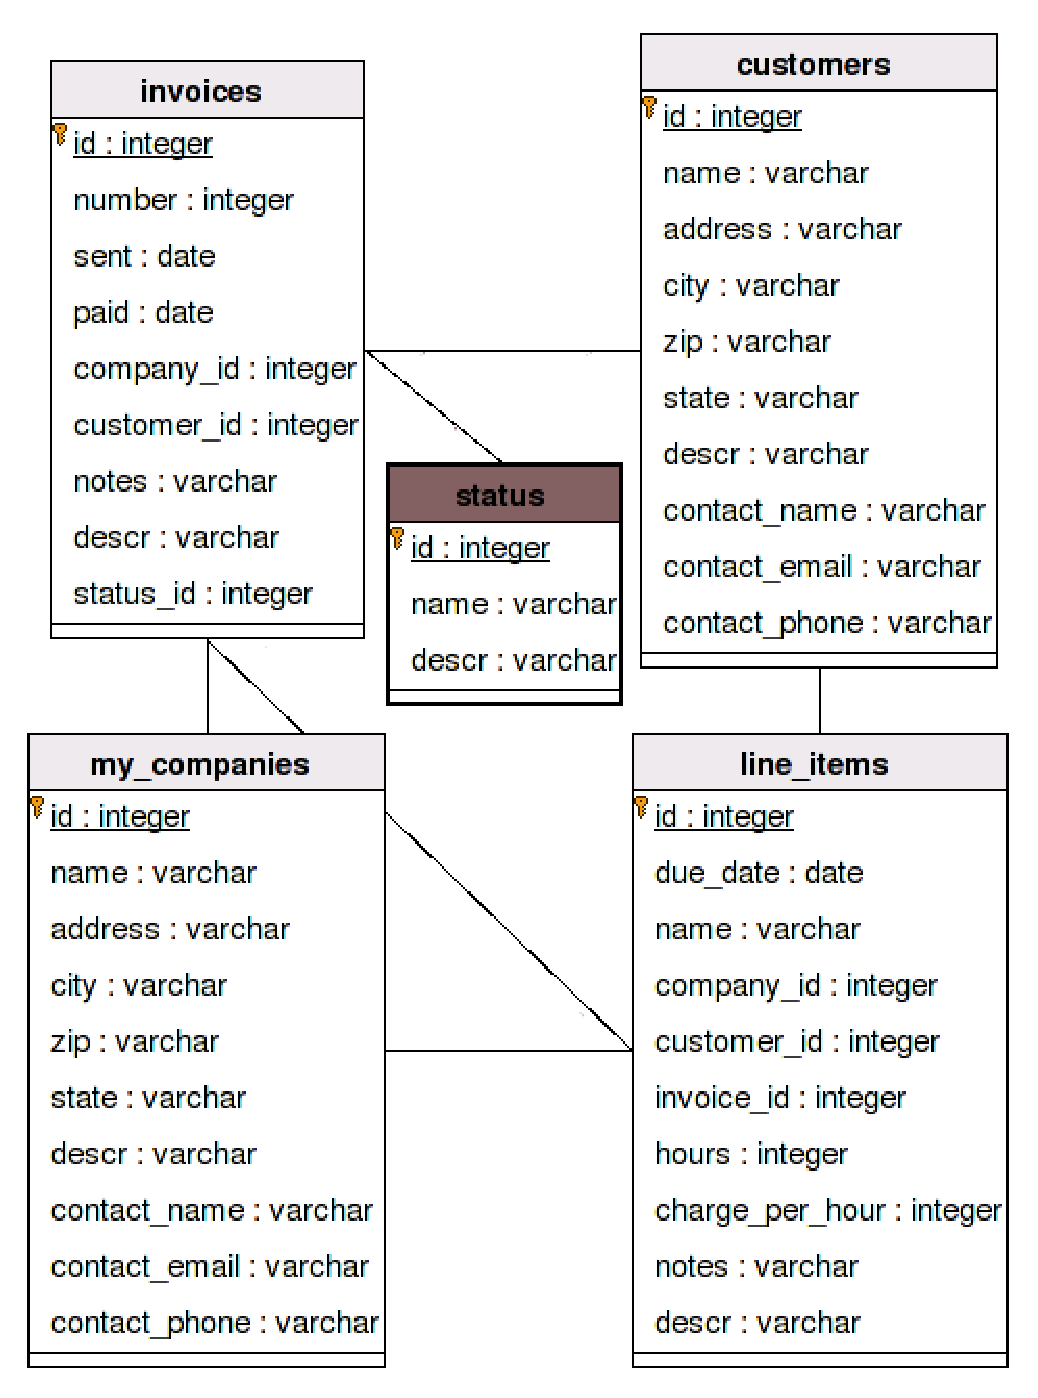
\includegraphics[height=6in]{billing_model}
\caption{Original billing application data model.}
\label{fig:billing_model}
\end{figure}

\section{Bigtop File for Billing App}

While I could walk you through using bigtop and tentmaker to build this
data model, that wouldn't add much to previous chapters, see for example
Chapter \ref{chap:simpleex}.  Instead, I'll show you the finished bigtop
file I made with bigtop, tentmaker, and my favorite editor.  While tentmaker
is great for getting started, it is often easier to move to a text editor to
fill in large chunks of repetitive descriptions.  Here is the finished result,
over 300 lines of it:

\begin{verbatim}
config {
    engine          CGI;
    template_engine TT;
    Init            Std             {}
    CGI             Gantry          { with_server 1; gen_root 1; flex_db 1; }
    SQL             Postgres        {}
    SQL             MySQL           {}
    SQL             SQLite          {}
    Control         Gantry          { dbix 1; }
    Model           GantryDBIxClass {}
    SiteLook        GantryDefault   {}
}
app Billing {
    authors `Phil Crow`, `Tim Keefer`;
    config {
        dbconn           `dbi:SLQite:dbname=app.db` => no_accessor;
        template_wrapper `genwrapper.tt`  => no_accessor;
    }
    table    my_company      {
        foreign_display `%name`;

        field id { is int4, primary_key, auto; }
        field name {
            is             varchar;
            label          Name;
            html_form_type text;
        }
        field address {
            is             varchar;
            label          Address;
            html_form_type text;
        }
        field city {
            is             varchar;
            label          City;
            html_form_type text;
        }
        field state {
            is             varchar;
            label          State;
            html_form_type text;
        }
        field zip {
            is             varchar;
            label          Zip;
            html_form_type text;
        }
        field description {
            is                 varchar;
            label              Description;
            html_form_type     text;
            html_form_optional 1;
        }
        field contact_name  {
            is                 varchar;
            label              `Contact Name`;
            html_form_type     text;
        }
        field contact_email {
            is                 varchar;
            label              `Contact Email`;
            html_form_type     text;
        }
        field contact_phone {
            is                 varchar;
            label              `Contact Phone`;
            html_form_type     text;
        }
        data
            name => `Crow Motors`,
            address => `12 E. Main`,
            city => `Paxton`,
            state => `NE`,
            zip => 69155,
            description => `Car and Implement Sales and Service`,
            contact_name => `EJ`,
            contact_email => `ej@example.com`,
            contact_phone => `1-800-CROW-MOT`;
    }
    table    customer         {
        foreign_display `%name`;

        field id { is int4, primary_key, auto; }
        field name {
            is             varchar;
            label          Name;
            html_form_type text;
        }
        field address {
            is             varchar;
            label          Address;
            html_form_type text;
        }
        field city {
            is             varchar;
            label          City;
            html_form_type text;
        }
        field state {
            is             varchar;
            label          State;
            html_form_type text;
        }
        field zip {
            is             varchar;
            label          Zip;
            html_form_type text;
        }
        field description {
            is                 varchar;
            label              Description;
            html_form_type     text;
            html_form_optional 1;
        }
        field contact_name  {
            is                 varchar;
            label              `Contact Name`;
            html_form_type     text;
            html_form_optional 1;
        }
        field contact_email {
            is                 varchar;
            label              `Contact Email`;
            html_form_type     text;
            html_form_optional 1;
        }
        field contact_phone {
            is                 varchar;
            label              `Contact Phone`;
            html_form_type     text;
            html_form_optional 1;
        }
        data
            name => `Groover Nordqvist`,
            address => `502 E. Third`,
            city => `Paxton`,
            state => `NE`,
            zip => 69155,
            description => `Prime Customer`,
            contact_name => `Groover`,
            contact_email => `gnordqvist@example.com`,
            contact_phone => `Unlisted`;
    }
    table    line_item        {
        foreign_display `%name`;

        field id { is int4, primary_key, auto; }
        field due_date {
            is               date;
            label            `Due Date`;
            date_select_text Select;
            html_form_type   text;
        }
        field name {
            is               varchar;
            label            Name;
            html_form_type   text;
        }
        field invoice {
            is                 int4;
            label              `Invoice Number`;
            refers_to          invoice;
            html_form_type     select;
        }
        field hours {
            is                 int4;
            label              Hours;
            html_form_type     text;
        }
        field charge_per_hour {
            is                 int4;
            label              Rate;
            html_form_type     text;
        }
        field notes {
            is                 text;
            label              `Notes to Customer`;
            html_form_type     textarea;
            html_form_optional 1;
            html_form_rows     4;
            html_form_cols     50;
        }
        field description {
            is                 text;
            label              `Notes to Self`;
            html_form_type     textarea;
            html_form_optional 1;
            html_form_rows     4;
            html_form_cols     50;
        }
    }
    table    invoice          {
        foreign_display `%number`;

        field id { is int4, primary_key, auto; }
        field number {
            is                 varchar;
            label              Number;
            html_form_type     text;
        }
        field status {
            is                 int4;
            label              Status;
            refers_to          status;
            html_form_type     select;
        }
        field sent {
            is                 date;
            label              `Sent On`;
            date_select_text   `Popup Calendar`;
            html_form_type     text;
            html_form_optional 1;
        }
        field paid {
            is                 date;
            label              `Paid On`;
            date_select_text   `Popup Calendar`;
            html_form_type     text;
            html_form_optional 1;
        }
        field my_company {
            is                 int4;
            label              `My Company`;
            refers_to          my_company;
            html_form_type     select;
        }
        field customer {
            is                 int4;
            label              Customer;
            refers_to          customer;
            html_form_type     select;
        }
        field notes {
            is                 text;
            label              `Notes to Customer`;
            html_form_type     textarea;
            html_form_optional 1;
            html_form_rows     4;
            html_form_cols     50;
        }
        field description {
            is                 text;
            label              `Notes to Self`;
            html_form_type     textarea;
            html_form_optional 1;
            html_form_rows     4;
            html_form_cols     50;
        }
    }
    table    status            {
        foreign_display `%name: %description`;

        field id { is int4, primary_key, auto; }
        field name {
            is             varchar;
            label          Name;
            html_form_type text;
        }
        field description {
            is             varchar;
            label          Description;
            html_form_type text;
        }

        data name => `Working`, description => `Work in Progress, NOT Billed`;
        data name => `Sent`,    description => `Mailed to Customer`;
        data name => `Paid`,    description => `Payment Received`;
    }
    controller Status is AutoCRUD {
        controls_table   status;
        rel_location     status;
        text_description status;
        page_link_label  Status;
        method do_main is main_listing {
            title            `Status`;
            cols             name;
            header_options   Add;
            row_options      Edit, Delete;
        }
        method form is AutoCRUD_form {
            form_name        status;
            fields           name, description;
            extra_keys
                legend     => `$self->path_info =~ /edit/i ? 'Edit' : 'Add'`;
        }
    }
    controller Company is AutoCRUD {
        controls_table   my_company;
        rel_location     company;
        text_description company;
        page_link_label  Companies;
        method do_main is main_listing {
            title            `My Companies`;
            cols             name, contact_phone;
            header_options   Add;
            row_options      Edit, Delete;
        }
        method form is AutoCRUD_form {
            form_name        company;
            all_fields_but   id;
            extra_keys
                legend     => `$self->path_info =~ /edit/i ? 'Edit' : 'Add'`;
        }
    }
    controller Customer is AutoCRUD {
        controls_table   customer;
        rel_location     customer;
        text_description customer;
        page_link_label  Customers;
        method do_main is main_listing {
            title            `Customers`;
            cols             name, contact_name, contact_phone;
            header_options   Add;
            row_options      Edit, Delete;
        }
        method form is AutoCRUD_form {
            form_name        customer;
            all_fields_but   id;
            extra_keys
                legend     => `$self->path_info =~ /edit/i ? 'Edit' : 'Add'`;
        }
    }
    controller LineItem is AutoCRUD {
        controls_table   line_item;
        rel_location     lineitem;
        uses             Gantry::Plugins::Calendar;
        text_description `line item`;
        page_link_label  `Line Items`;
        method do_main is main_listing {
            title            `Line Items`;
            cols             name, due_date;
            header_options   Add;
            row_options      Edit, Delete;
        }
        method form is AutoCRUD_form {
            form_name        line_item;
            all_fields_but   id;
            extra_keys
                legend     => `$self->path_info =~ /edit/i ? 'Edit' : 'Add'`,
                javascript => `$self->calendar_month_js( 'line_item' )`;
        }
    }
    controller Invoice is AutoCRUD {
        controls_table   invoice;
        rel_location     invoice;
        uses             Gantry::Plugins::Calendar;
        text_description invoice;
        page_link_label  Invoices;
        method do_pdf   is stub {
            extra_args   `$id`;
        }
        method do_main is main_listing {
            title            `Invoices`;
            cols             number, customer, status;
            header_options   Add;
            row_options
                Tasks => `"/lineitem/main/$id"`, PDF, Edit, Delete;
        }
        method form is AutoCRUD_form {
            form_name        invoice;
            all_fields_but   id;
            extra_keys
                legend     => `$self->path_info =~ /edit/i ? 'Edit' : 'Add'`,
                javascript => `$self->calendar_month_js( 'invoice' )`;
        }
    }
}
\end{verbatim}

There is one notable feature of this bigtop file. The \verb+status+,
+\verb+customer+ and \verb+my_company+ tables use data statements.  In
\verb+status+ they provide the actual data for the table.  Users will be
able to add, edit, and delete in the table, but these are meant to be
useable as a production starting point.  The other two use data statements
to supply test data.  This softens the blow of discarding a database during
development.  Normally I would remove the data statements before building
the final schema files.  But even when I forget, the pain is limited to
deleting two rows from the production database.

You cannot currently manage data statements with tentmaker.  But it will
not alter the ones you put in with an editor, except to cannocalize whitespace.
Each data statement begins with \verb+data+, then has a comma separated
list of field name/value pairs, where the field names and values are separated
by \verb+=>+.  The values must be properly quoted.  The statement ends with
a semi-colon.  You may use as many data statements as you like.
Each one becomes a separate INSERT INTO statement.

Turning the above into a working app is as simple as the example in Chapter
\ref{chap:simpleex}:

\begin{verbatim}
bigtop --create billing.bigtop all
cd Apps-Billing
sqlite app.db < docs/schema.sqlite
./app.server
\end{verbatim}

\section{Finishing the Bills}

Of course, the app so far is generic.  It does not know how to make PDF
invoices or even how to display the tasks associated with an invoice, but
it does all the other tedious parts.

So, let's finish it.  There are only a few remaining pieces, both start in
the Invoice controller.

\subsection*{Showing Tasks for One Invoice}

First, let's link invoices to their tasks.  From the bigtop file in the
previous section, you can see that the generated row option for Tasks points
to the Line Item controller:

\begin{verbatim}
        options => [
            {
                text => 'Tasks',
                link => "/lineitem/main/$id",
            },
        #...
\end{verbatim}

The idea is to call the \verb+do_main+ in the Line Item controller, passing
it the invoice number, to which it should limit the line items displayed.
For that to work, we need to modify the \verb+do_main+ Bigtop generated
for us.  The generated one is almost right.  So, I copied it from
GEN/LineItem.pm to LineItem.pm.  There is no need to modify the bigtop file
or remove it from the GEN module.  Stub controllers inherit from their
generated modules, so we can simply override the method.

In order for my new \verb+do_main+ method to work, I need to use a couple
of additional modules at the top of the \verb+LineItem+ controller:

\begin{verbatim}
use Billing::Model::line_item qw( $LINE_ITEM );
use Billing::Model::invoice   qw( $INVOICE   );
\end{verbatim}

Actually, the first of those was already present, but I removed some
whitespace to make it prettier.

Here is the new \verb+do_main+, lines marked with # * are new, those
with M are modified:

\begin{verbatim}
#-----------------------------------------------------------------
# $self->do_main( [ $invoice_id ] )                                 # M
#-----------------------------------------------------------------
sub do_main {
    my ( $self, $invoice_id ) = @_;                                 # M

    my $only_one_invoice = 0;                                       # *
    my $title            = 'Line Items';                            # *
    if ( defined $invoice_id ) {                                    # *
        $only_one_invoice = 1;                                      # *
        my $invoice = $INVOICE->gfind( $self, $invoice_id );        # *
        $title .= ' for Invoice ' . $invoice->foreign_display();    # *
    }                                                               # *

    $self->stash->view->template( 'results.tt' );
    $self->stash->view->title( $title );

    my $retval = {
        headings       => [
            'Name',
            'Due Date',
            'Invoice',
        ],
        header_options => [
            {
                text => 'Add',
                link => $self->location() . "/add",
            },
        ],
    };

    my $schema = $self->get_schema();
    my @rows   = $LINE_ITEM->get_listing( { schema => $schema } );

    ROW:                                                            # *
    foreach my $row ( @rows ) {
        my $id = $row->id;

        next ROW if ( $only_one_invoice and $id != $invoice_id );   # *

        push(
            @{ $retval->{rows} }, {
                data => [
                    $row->name,
                    $row->due_date,
                    $row->invoice->foreign_display(),
                ],
                options => [
                    {
                        text => 'Edit',
                        link => $self->location() . "/edit/$id",
                    },
                    {
                        text => 'Delete',
                        link => $self->location() . "/delete/$id",
                    },
                ],
            }
        );
    }

    $self->stash->view->data( $retval );
} # END do_main
\end{verbatim}

The main changes are at the top.  First, I altered the opening commit to
show future coders that invoice id is an optional parameter.   Then, inside
the sub, I check the value.  If it is true, I set a flag, get the invoice
with that id, and append its name to the title.

I made only two other changes: I gave the line item walking loop a label
and I added a test which skips rows for other invoices, if we care.  Remember
that users may hit the page directly.  Then they presumably want to see
all the tasks.

\subsection*{How Many Tasks Must I Do?}

For shear fun, I decided that the Tasks link should indicate how many
tasks are associated with the invoice.  While this is clearly not necessary,
it does show some addtional techniques, further I've done it for other apps
to the delight of my users.

This change also involves overriding \verb+do_main+, but less dramatically.
The new Invoice.pm \verb+do_main+ dispatches to the parent version in the
GEN module, then modifies it:

\begin{verbatim}
#-----------------------------------------------------------------
# $self->do_main(  )
#-----------------------------------------------------------------
sub do_main {
    my $self = shift;

    $self->SUPER::do_main();

    my $rows             = $self->stash->view->data()->{ rows };
    my $line_item_counts = $LINE_ITEM->get_count( $self );

    foreach my $row ( @{ $rows } ) {
        my $task_option = $row->{ options }[0];
        my $id          = ( split /\//, $task_option->{ link } )[-1];
        my $count       = $line_item_counts->{ $id } || 0;
        $task_option->{ text } .= " ($count)";
    }
}
\end{verbatim}

When the SUPER version finishes, the template data is in
\verb+$self->stash->view->data()+.  In particular, we are interested in the
\verb+rows+ hash key.  For each row, we want to add a count of tasks after
the link text `Tasks'.  First, we need to know how many tasks there are for
this invoice.  The neatest way to find out is to ask the model.  Later we
will see how it calculates these counts.  For now, it is enough to know
that they come back in a hash reference keyed by invoice row id.

Once we have the data from the parent (GEN) module and a count of all the
tasks collated by invoice, we are ready to walk through the output rows.
Each row is itself a hash.  One key, the one we care about, is `options.'
It stores the links and locations for the right hand column.  Users click
these to navigate.  Usually there are only Edit and Delete links.  Recall
from above that this app also has Tasks and PDF.

The Tasks link comes first (element zero in the array).  We are interested
in the text, but we must retrieve the row id from the link.  That id is
the last element of the URL, hence the split on slashes using only the item
at index -1.  With the id, we can look up the task count for the invoice.
Finally, we can append the the count (in parentheses) to the link text.

The remaining piece counts the tasks, grouping them by invoice id.  It is
implemented in a method in the model stub.  Thus, the following code goes
in \verb+lib/Billing/Model/line_item.pm+:

\begin{verbatim}
sub get_count {
    my $class       = shift;
    my $gantry_site = shift;

    my %retval;

    my @line_items = $class->gsearch( $gantry_site );

    foreach my $line_item ( @line_items ) {
        $retval{ $line_item->invoice->id }++;
    }

    return \%retval;
}
\end{verbatim}

Gantry's DBIx::Class model base class provides \verb+gsearch+ and other
helper methods to save some typing.  This one does a search on the table.
Since no args were provided beyond the site object (which knows how to
get the schema), all rows are returned.

A quick loop through the line items collects the counts in a hash, which
is returned as a hash reference.

\subsection*{Printable Invoices}

With a realitively easy way for users to examine task/invoice connections,
it is time to actually make invoices.  The full version that ships with
Bigtop has a PDF generator in it.  I'm leaving that out here, because it
is large and repetative.  Instead, I'm going to make a plain text invoice.
It won't look as nice, but it will save almost a hundred lines of code
(most of those lines are PDF positioning statements).  Even so, these routines
are rather large and are largely uninteresting.

So that the link structure will not break, I'm still calling the method
\verb+do_pdf+.  Feel free to change the links, etc.

\begin{verbatim}
#-----------------------------------------------------------------
# $self->do_pdf( $id )
#-----------------------------------------------------------------
sub do_pdf {
    my ( $self, $id ) = @_;

    # pull variables out of invoice row ready for here doc
    my $invoice     = $INVOICE->gfind( $self, $id );
    my $invoice_num = $invoice->number;
    my $sent        = $invoice->sent;
    my $description = $invoice->description || '';

    $description    = "\n$description\n" if $description;

    # my company data
    my %corp_data;

    foreach my $column qw( name address city state zip contact_phone ) {
        $corp_data{ $column } = $invoice->my_company->$column();
    }

    # customer data
    my %cust_data;
    foreach my $column
            qw( name address city state zip contact_phone contact_name )
    {
        $cust_data{ $column } = $invoice->customer->$column();
    }

    # tasks, pass the buck
    my ( $task_output, $total ) = $self->_task_output( $id );

    my $retval = << "EO_Invoice";
Billed By:
$corp_data{ name }
$corp_data{ address }
$corp_data{ city }, $corp_data{ state } $corp_data{ zip }
$corp_data{ contact_phone }

Billed To:
$cust_data{ name }
$cust_data{ address }
$cust_data{ city }, $cust_data{ state } $cust_data{ zip }
$cust_data{ contact_phone }
Attn: $cust_data{ contact_name }

Invoice Number: $invoice_num Invoice Date: $sent $description

Date         Hours    Rate/hr    Total   Task
$task_output
_______________________________________________________________________

Total Amount Due: $total

Invoice due upon receipt.
EO_Invoice

    $self->template_disable( 1 ); 		# turn off templating
    $self->content_type( 'text/plain' );

    return $retval;
}
\end{verbatim}

This generates all of the output except the actual task list, which is below.
First, I retrieve the invoice to be made printable, using the \verb+gfind+
method provided by Gantry's DBIx::Class base module.  From it I fish out
various strings to go on the bill.  I want to fish first instead of trying
to call methods inside the here doc.

Then, I fish the company and customer data from the invoice row object.
Once the data is fished out, it is a simple matter of here doc construction.
The tasks are presented via their own method:

\begin{verbatim}
sub _task_output {
    my ( $self, $id ) = @_;

    my @tasks = $LINE_ITEM->gsearch( $self, { invoice => $id } );

    my @rows;
    my $total       = 0;
    my $space       = ' ';

    foreach my $task ( @tasks ) {
        my $row_amount = $task->hours() * $task->charge_per_hour();

        $total        += $row_amount;

        my $row_output = $task->due_date()        . $space x 4;
        $row_output   .= $task->hours()           . $space x 8;
        $row_output   .= $task->charge_per_hour() . $space x 9;
        $row_output   .= $row_amount              . $space x 10;
        $row_output   .= $task->name();

        push @rows, $row_output;
    }
    my $task_output = join "\n", @rows;
    
    return $task_output, $total;
}
\end{verbatim}

Since each task will go on one line, the fishing can be done directly into
the output.  Note that the cost of each line item is calculated here and
a total is returned along with the text for each line item.

Now, when the user clicks Tasks on the invoice page, they will go to the
Line Item controller, but see only the tasks for that invoice.  When the
user clicks PDF, they will get a new page with the text ready for inclusion
in a sickly looking email.  The genuine PDF version looks a bit better.

Keep in mind that all preceding code was written for programmer efficiency
only.  Most of the code could be written to minimize other costs, like
run time.  If the app is successful, expect to be required to make such
changes over time.  But, I always start with getting something that works,
which is easy to read.  Only after a speed problem emerges do I shift from
optimizing for my time to optimizing for the computer's time.

In this chapter, we have seen how to customize a Bigtop generated app with
a minimum of new code  While that may not be the best use a computer's
time for large apps, it is quite a good use of our time for most apps.

The next chapter presents another case study beginning with Bigtop and ending
with custom code.  This time, concepts such as Apache basic auth and
many-to-many relationships between tables appear.
